\section{Points of interest detection}

% TODO: move to the introduction?
In this section, the term \emph{training image} refers to the reference image to which a \emph{test image} can be compared. The training image is stored in the search database, whereas the test image is the image one is trying to match against the images in the database.

\subsection{Scale invariance and scale space}

When identifying points of interest, or features, in the training image, it is important that those features can be detected even if the image is scaled. Indeed, the test image can have a different zoom level. Feature detection is thus done in scale space \cite{Lindeberg98featuredetection}. A two dimensional signal, such as an image, $f: \mathbb{R}^2 \to \mathbb{R}$, is represented in scale space $L: \mathbb{R}^2 \times \mathbb{R}_+ \to \mathbb{R}$ by
\begin{equation}
L(x,y;t) = g(x,y;t) \ast f(x,y)
\end{equation}
where $g: \mathbb{R}^2 \to \mathbb{R}$ is the Guassian kernel with variance $t=\sigma^2$
\begin{equation}
g(x,y;t) = \frac{1}{2 \pi t} e ^ \frac{-(x^2+y^2)}{2t}
\end{equation}

Using the properties of convolution, one can compute the scale space derivative at scale $t$ by convolving the image with the derivative of the Gaussian kernel:
\begin{equation}
    L_{x^\alpha y^\beta} (x,y;t) = \partial _{x^\alpha y^\beta} L(x,y;t) = \partial _{x^\alpha y^\beta} (g(x,y;t) \ast f(x,y)) = (\partial _{x^\alpha y^\beta} g(x,y;t)) \ast f(x,y)
\end{equation}
Here $\alpha$ and $\beta$ are the orders of differentiation with respect to $x$ and $y$ respectively.

\subsection{Blob detection with the determinant of the Hessian}

In \cite{Lindeberg93detectingsalient} Lindeberg describes a method for detecting blob-like structures from the scale space representation of an image. He informally defines a blobs at a defined scale as ``smooth regions which are brighter or darker than the background and stand out from their surroundings''. These regions typically appear at multiple scales. If they can be uniquely linked accross the scales they form a scale space blob \cite{Lindeberg93detectingsalient}. The extrema at scale $t$ give the locations of blobs.

One method to find the extrema in a multivariate function $f$ is to find all solutions $x_0, ... x_i, ... x_n$ to $\vec\nabla f = \vec0$ and then compute the determinant of the Hessian matrix evaluated at each point $x_i$. If the determinant is positive, then $x_i$ is a local minimum, if it is negative, $x_i$ is a local maximum. A determinant of 0 indicates a saddle point at $x_i$.

In the case of blob detection, the analyzed function is the scale space representation of the image. As such, the equations are as follows \cite{Lindeberg93detectingsalient}.

A critical point $x_0 \in \mathbb{R}$ at scale $t_0 \in \mathbb{R}_+$ satisfies:

\begin{equation}
    \nabla L\rvert_{(x_0; t_0)} =
    \begin{bmatrix}
        L_{x} \\ L_{y}
    \end{bmatrix} \Bigg\rvert_{(x_0; t_0)} =
    \begin{bmatrix}
        0 \\ 0
    \end{bmatrix}
\end{equation}

The determinant of the Hessian matrix is:

\begin{equation}
    det(H(\mathbf{x},t)) =
    \begin{vmatrix}
        L_{xx}(\mathbf{x},t) & L_{xy}(\mathbf{x},t) \\
        L_{xy}(\mathbf{x},t) & L_{yy}(\mathbf{x},t)
    \end{vmatrix}
    =
    L_{xx}(\mathbf{x},t) L_{yy}(\mathbf{x},t) - (L_{xy}(\mathbf{x},t))^2
\end{equation}

\subsection{Integral images}

For an input image $i$, \cite{Viola01rapidobject} defines the integral image $I$ as a two dimensional array which at position $\mathbf{x} = (x,y)$ contains the sum of the intensities of all pixels above and to the left of $\mathbf{x}$.
\begin{equation}
I(x,y) = \sum_{\begin{smallmatrix} x' \le x \\ y' \le y\end{smallmatrix}} i(x',y')
\end{equation}
This assumes the coordinate system is as usually defined in computer graphics: the origin is at the upper left corner, the y coordinates increase downwards, the x coordinates increase to the right.

\begin{figure}
    \centering
    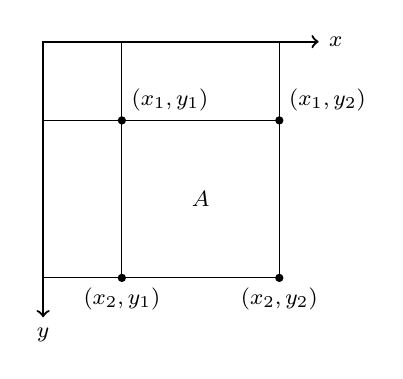
\begin{tikzpicture}[font=\footnotesize]
        \draw [<->,thick] (0,-3.5) node (yaxis) [below] {$y$} |- (3.5,0) node (xaxis) [right] {$x$};
        \draw (1,0) coordinate (a1) -- (1,-3) coordinate (a2);
        \draw (0,-1) coordinate (b1) -- (3,-1) coordinate (b2);
        \draw (0,-3) coordinate (c1) -- (3,-3) coordinate (c2);
        \draw (3,0) coordinate (d1) -- (c2);
        \coordinate (A) at (intersection of a1--a2 and b1--b2);
        \fill (A) circle (1.5pt)  node [above right] {$(x_1, y_1)$};
        \fill (b2) circle (1.5pt) node [above right] {$(x_1, y_2)$};
        \fill (a2) circle (1.5pt) node [below] {$(x_2, y_1)$};
        \fill (c2) circle (1.5pt) node [below] {$(x_2, y_2)$};
        \draw (2,-2) node {$A$};
    \end{tikzpicture}
    \caption{
        Using the integral image $I$, the sum of pixels in the area $A$ of the source image can be expressed as
        $I(x_2,y_2) -  I(x_1,y_2) - I(x_2,y_1) + I(x_1,y_1)$
        \label{fig:integral_images}
    }
\end{figure}

Integral images make computing intensity sums with arbitrary rectangular areas in an image efficient. Figure~\ref{fig:integral_images} gives an example.

\subsection{Fast Hessian blob detection using box filters and integral images}

Convolution with Gaussian derivatives is computationaly expensive. In \cite{Bay06surf:speeded} Bay et al. approximate the second order Gaussian derivatives with box filters (see figure~\ref{fig:gaussian_derivatives}). Because box filters are constitued of regions with a common weight, convolution can be expressed using the procomputed sums from the integral image.


\begin{figure}
    \centering
    \includegraphics[height=0.3\textheight]{img/gaussian-kernel-derivatives}
    \caption{
        The top row shows the cropped second order derivatives of a Gaussian kernel with variance $\sigma^2=1.2$ (from left to right:
        $\partial_{xx} g(x,y)$, $\partial_{yy} g(x,y)$, $\partial_{xy} g(x,y)$).
        The bottom row shows the corresponding (9x9) box filter approximations.
        \label{fig:gaussian_derivatives}
    }
\end{figure}

The approximations of $L_{xx}$, $L_{yy}$, $L_{xy}$ are respectively denoted $D_{xx}$, $D_{yy}$, $D_{xy}$.



(TODO: write about how filters grow)

With $\mathbf{x} = (x,y)$
\begin{equation}
    H(\mathbf{x},t)_{approx} = 
    \begin{bmatrix}
        D_{xx}(\mathbf{x},t) & D_{xy}(\mathbf{x},t) \\
        D_{xy}(\mathbf{x},t) & D_{yy}(\mathbf{x},t)
    \end{bmatrix}
\end{equation}

Bay at al. balances the weight of the expressions in the determinant of this approximation as follows
\begin{equation}
    det(H_{approx}) = D_{xx} D_{yy} - (w D_{xy})^2
\end{equation}
The weight $w$ is defined as 
\begin{equation}
w(t,s) = \frac{\left|L_{xy}(t)\right|_F \left|D_{xx}(s)\right|_F}{\left|L_{xx}(t)\right|_F \left|D_{xy}(s)\right|_F}
\end{equation}
where $t$ is the scale, $s$ is the filter size and $\left|\cdot\right|_F$ is the Frobenius norm, $\left|A\right|_F=\sqrt{\sum_{i=1}^m\sum_{j=1}^n |a_{ij}|^2}$.
For instance, the weight for a 9x9 filter and a scale of 1.2 is $w(t=1.2, s=9) \simeq 0.9$.

(TODO: write about octaves?)

(TODO: write about finding the maximum determinant of hessian in a 3x3 neighbourhood)

(TODO: write about interpolation)
\cite{Brown02invariantfeatures}:

\begin{equation}
\end{equation}

